\documentclass[12pt]{article}

%% Language and font encodings
%\usepackage[english]{babel}
%\usepackage[utf8x]{inputenc}
%\usepackage[T1]{fontenc}
\usepackage[margin=1in]{geometry}

%% Sets page size and margins
%\usepackage[a4paper,top=3cm,bottom=2cm,left=3cm,right=3cm,marginparwidth=1.75cm]{geometry}

%% Useful packages
\usepackage{amsmath}
\usepackage{graphicx}
%\usepackage[colorinlistoftodos]{todonotes}
%\usepackage[colorlinks=true, allcolors=blue]{hyperref}

\usepackage{caption}
\usepackage{subcaption}
\usepackage{xcolor}

\graphicspath{{res/}}

\title{Lab 2}
\author{Lukas Finkbeiner}

\begin{document}

\maketitle

\begin{abstract}

We investigated the hyperfine hydrogen transition by calibrating our measurements to thermal noise and by averaging over many blocks of data taken in optimal time windows of the day. We investigated the speed of light using waveguides (\textcolor{red}{How do they work?}). Our Chi-Squared analysis is completely deficient because our data were taken too broadly to show noticeable inconsistencies.

This is a great place to have a to-do section, because I prefer to write abstracts at the end of the writing process.

\quad * Ask Professor about the permissions thing (page 3), to make sure there are no technical difficulties.

\textcolor{red}{Figure out how to make the section headers smaller. They are taking up far too much space.}

\end{abstract}

% No need to re-derive anything!!

\section{Introduction and Background}

\textcolor{red}{Block diagram of the telescope electronics}. Fortunately, it seems like the professor took care of most of this for you in lecture, February 11.

% Leave the waveguide equations for the `models' section

% 3. The equations for the two waveguides; scipy.optimize.fmin

\section{Methods}

To place our test signal in the upper and lower sidebands, we use these two frequencies. To put the hydgrogen in the upper and lower sidebands, we set the first local oscillator to these other two frequencies.

\section{Observations}

As a preface, I may want to include commentary on how I had to manually alter the data, based on readings from the oscilloscope, in order to account for the imbalance in picoscope inputs?? I think not!

% The times of observation and why that matters.

% 1. scrap for time: initial calibration results. Here is a test signal. ``Our setup works!''
% source of error: angles are not aligned well. 10% error becomes... 25%? in power plot. I do not remember.

% scrap for time: justify the use of mean vs median

% acknowledge that from now on, you are setting the y limits to ignore both the central
% spike as well as the bunny ears

% acknowledge that, for shape spectra, we are deliberately ignoring the spikes at +- 2 MHz

% 2. initial H1 observations: on-line and off-line, to get the line shape
% difference between mean and median

\begin{figure}
\centering
\begin{minipage}{.45\textwidth}
	\centering
	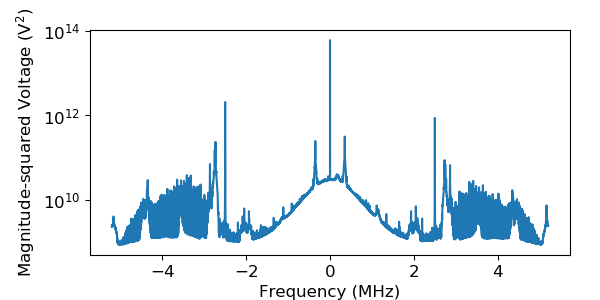
\includegraphics[width=\linewidth]{limits_justification}
	\captionof{figure}{A semi-log plot over the range of frequencies sampled. We assume that our 2 MHz low-pass filter works, so we will dismiss the signals farther than 2 MHz from the center. Additionally, the large central spike and smaller `bunny ear' spikes ($\pm$.5 MHz) appear on all data sets as persistent interference; we partially ignore these by limiting the y-axis.}
	\label{fig:on_limits}
\end{minipage} \hfill%
\begin{minipage}{.45\textwidth}
	\centering
	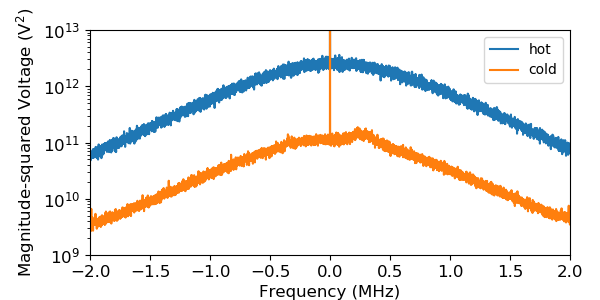
\includegraphics[width=\linewidth]{thermal}
	\captionof{figure}{The `hot' data correspond to three humans standing in front of the collector. The `cold' data correspond to the collector pointing up at the cold sky. The noise is not an issue because of its regularity: observe the even discrepancy between the curves over the domain of interest.}
	\label{fig:thermal}
\end{minipage}
\end{figure}

\begin{figure}
\centering
\begin{minipage}{.5\textwidth}
	\centering
	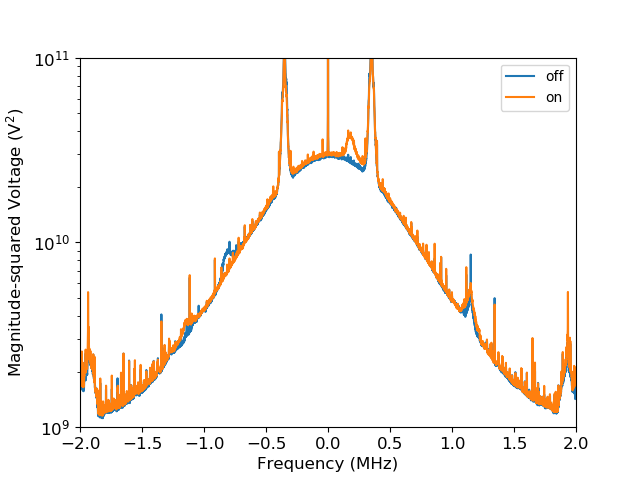
\includegraphics[width=\linewidth]{up_on_off}
	\caption{Watch it move.}
	\label{fig:up_on_off}
\end{minipage}%
\begin{minipage}{.5\textwidth}
	\centering
	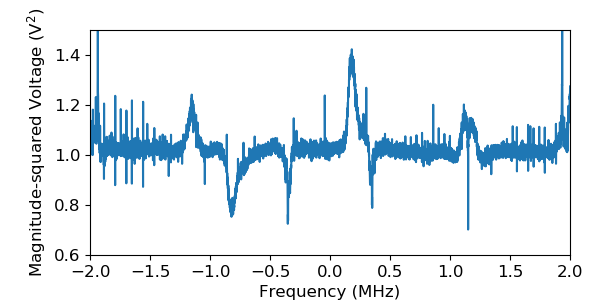
\includegraphics[width=\linewidth]{up_shape}
	\caption{\textcolor{red}{This one is not helpful. Replace it with the final, calibrated spectrum, thermal power units.}}
	\label{fig:up_shape}
\end{minipage}
\end{figure}

% 3. Gain observation: overplot hot and cold

% 4. Plot waveguide results, at least for the xband, to talk about how weird everything is.
% caliper measurement for a. 'This is what we hope to get from analysis'
% sources of error.

\section{Analysis}

% 1. The poly fit to the baseline

% 2. The Gaussian fits to the remaining curves

% 3. 

\section{Conclusions}


\section{Acknowledgments}

\textcolor{red}{You have to remedy your complete ignorance of BibTex}

\end{document}
